\documentclass{article}
\usepackage{graphicx}
\usepackage{amsmath}
\usepackage{float}
\title{Misurazione della refrattività del'acqua}
\author{Alessandro Di Meglio \\ Francesco Angelo Fabiano Antonacci}
\date{\today}
\begin{document}

\maketitle
\section{Scopo dell'esperienza}

Lo scopo dell'esperienza è quello di misurare la refrattività  dell'acqua mediante una lente cilindrica.

\section{Cenni teorici}

Data una lente la relazione tra f, ossia la distanza focale della lente, p ,la distanza tra il centro della lente e la sorgente luminosa, e q , la distanza tra il centro della lente e l'immagine messa a fuoco, è la legge dei punti coniugati:

\begin{equation}
\frac{1}{f}=\frac{1}{p}+\frac{1}{q}
\label{pucon}
\end{equation}

Ponendo $\frac{1}{p}=x$ ,  $\frac{1}{q}=y$ e $\frac{1}{f}=c$ otteniamo la seguente relazione:
\begin{equation}
y=c-x
\label{:)}
\end{equation}
 


Data una lente di raggio r costituita da un mezzo con un indice di rifrazione n, l'equazione del costruttore di lenti ci dà una relazione con la distanza focale:

\begin{equation}
\frac{1}{f}=(n-1)\frac{2}{r}(1-\frac{n-1}{n})
\label{lme}
\end{equation}

Da cui otteniamo l'equazione per stimare la refrattività $\eta$:

\begin{equation}
\eta=\frac{r}{2f-r}
\label{refr}
\end{equation}


\section{Apparato strumentale}

\subsection{Materiale Utilizzato}

Per l'esperienza sono stati utilizzati i seguenti strumenti:
\begin{itemize}

\item Schermo
\item Smartphone
\item Bottiglia cilindrica di vetro
\item Nastro adesivo
\item Filo
\end{itemize}


\subsection{Misure di lunghezza}
Per le misure di lunghezza è stato utilizzato un metro a nastro con risoluzione di 1 mm.



\section{Descrizione delle misure}

E' stata costruita la lente riempendo la bottiglia di acqua.
Sono stati compiuti 4 giri di spago attorno alla bottiglia, si è presa la lunghezza dello spago che ha avvolto la bottiglia.
E' stato fissato un metro  a nastro su un banco per poter prendere le coordinate degli oggetti del banco ottico.
E' stata posizionata la lente a una coordinata che è rimasta fissa per tutto l'esperimento.
E' stata attivata la torcia dello smartphone.
E' stato posizionato lo smartphone in successive posizioni; in ciascuna è  stata presa la distanza tra il centro della lente e lo schermo nella configurazione in cui la luce proiettata su esso era a fuoco.
E' stata dedicata particolare cura a tenere l'asse passante per la torcia e il centro della lente  parallelo al metro a nastro.

\subsection{Incertezze sulle misure di posizione}

Si veda la sezione \textbf{Cenni teorici} per la notazione usata.

\subsection{Incertezza su p}

L'incertezza sulla distanza tra telefono e centro della bottiglia è stata assunta 1[mm] a causa della risoluzione del metro a nastro.
E' stato verificato che l'effetto del possibile disallineamento (si veda:\textbf{Descrizione delle misure}) sulla misura di p influisce per meno di un decimo dell'incertezza dovuta alla risoluzione del metro a nastro. Per far ciò si è stimato che nel caso del p più piccolo $\sigma p \gg (\sqrt{p^2+\delta^2}-p)$ , dove per $\delta$ si è presa una stima per eccesso del possibile errore.

\subsection{Incertezza su q}

Per stimare l'incertezza su q è necessario tenere in considerazione il fatto che la cofigurazione in cui la lente è a fuoco avviene in un intorno di un punto.
Prendendo ripetute volte le misure si è osservato che questo intervallo è ampio dai 6 ai 4 [mm] dipendentemente dalla posizione.
Dunque, si stima come incertezza la somma in quadratura tra la deviazione standard della distribuzione uniforme su questo intervallo e la risolizione strumentale del metro a nastro.
Come nel caso precedente è stato verificato che l'effetto del possibile disallineamento sulla misura di q influisce per meno di un decimo dell'incertezza dovuta all'incertezza stimata. 

\subsection{Correlazione tra l'incertezza di p e quella di q}
\label{ind}
Le due incertezze sono debolmente correlate:come si è osservato nelle due sezioni precedenti sia p che q sono soggette a un errore determinato dal disallineamento rispetto al metro a nastro. 
Tuttavia si  è osservato che questo causa un errore trascurabile rispetto agli altri a cui è soggetta la misura.


\subsection{Incertezza su r}
L'incertezza sul raggio è l'incertezza sulla misura di 4 volte la circonferenza diviso $8\pi$.
E' ragionevole assumere che l'incertezza sulla misura della circonferenza sia la somma in quadratura dello spessore dei quattro giri e della risoluzione del metro a nastro.
Pertanto $\sigma r= 0.1$[mm].


\section{Analisi dei dati}
\subsection{Algoritmo di best fit}
Per trovare la distanza focale è stato fatto un fit ai minimi quadrati per la relazione (\ref{fiteq}) e non per la relazione (\ref{:)}).
Il parametro m ha il fine di scovare errori sistematici. Idealmente esso è $m=-1$.

\begin{equation}
	y=mx+c
	\label{fiteq}
\end{equation}

Le ipotesi per fare un fit ai minimi quadratici sono state verificate: le incertezze sulle x sono trascurabili, le incertezze sulle x e sulle y sono indipendenti.
Per poter trascurare l'errore sulle x ( $\sigma y \gg  \left| \frac{\delta f}{\delta x} \right| \sigma x $),  il fit è stato iterato più volte, 
utilizzando $\sigma y_{efficace}=\sqrt{\sigma y_{originaria}^2+(\frac{\delta f}{\delta x} \sigma x)^2}$ ,con $\frac{\delta f}{\delta x} $ ottenuta dall'iterazione precedente.


Sull'indipendenza delle incertezze si è discusso nella sezione( \ref{ind}).

In Table \ref{Pacciani} sono riportati i risultati dell'algoritmo di best-fit.
In Figure 1 sono presenti i dati sperimentali, la previsione del modello coi parametri di best-fit e il grafico dei residui.

		\begin{table}
			\centering
				\begin{tabular}{|c|c|c|}

					\hline
						$m$  & $c$[m] & $f$[m]\\
					\hline
			
						$-0.99\pm0.06$ & $11.3\pm0.2$ & $0.089\pm0.002$\\
					\hline
			
				\end{tabular}
					\caption{ Parametri ricavati dall'algoritmo di best-fit}
			\label{Pacciani}
		\end{table}		


\begin{figure}
	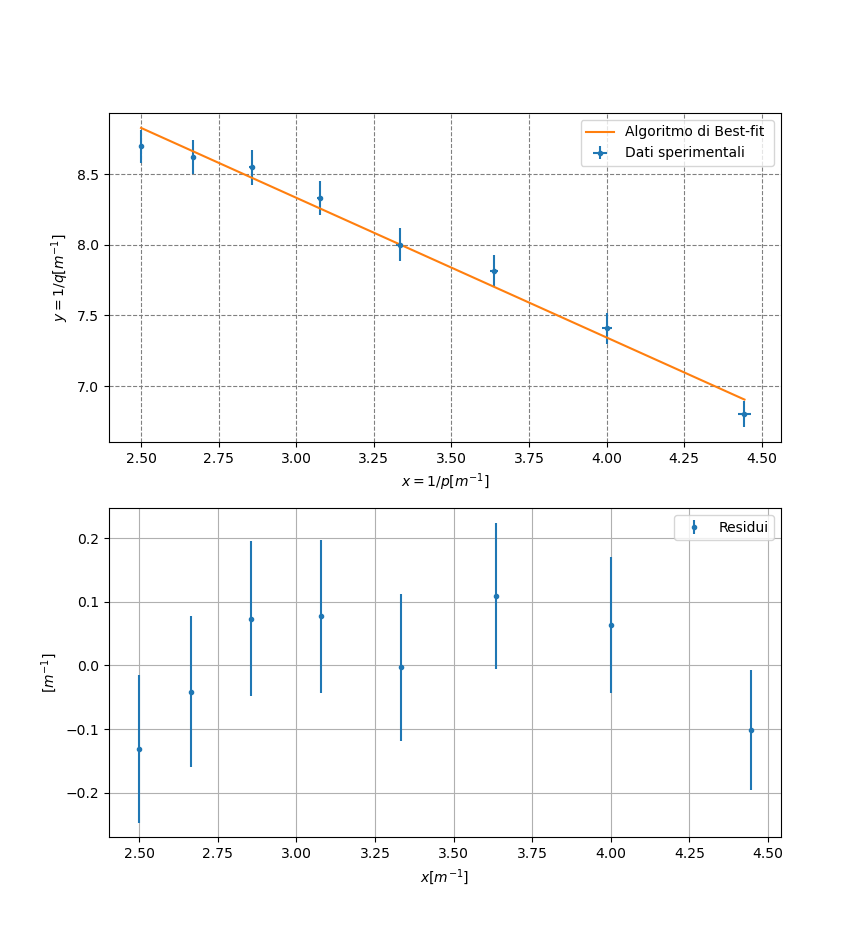
\includegraphics[width=\textwidth]{cylindricallens_grafico.png}
	\label{plottinobello}
	\caption{\\Sopra:Punti misurati e modello di (\ref{fiteq}) con i parametri dell'algoritmo di best-fit. \\ Sotto: Grafico dei residui.}
\end{figure}


\subsection{Test del $ X^2$ e p-value}
Il valore dei gradi di libertà è $\nu=6$: sono stati campionati 8 punti e sono stati 2 parametri nel modello (\ref{fiteq}). 
Il chi-quadro stimato è $X^2=4.6$.
Il p-value corrispondente è $p=0.1$.

\subsection{Errori sistematici}
Dal grafico dei residui non è evidente la presenza di errori sistematici.
Il valore stimato dall'algoritmo di best-fit per m  è compatibile con il valore dell'equazione (\ref{:)}).





\section{Conclusione}
\subsection{Misura di $\eta$}
Utilizzando l'equazione  ( \ref{refr} ) si ottiene $\eta$. 
In tabella (\ref{etameas} ) sono riportati i risultati.

		\begin{table}
			\centering
				\begin{tabular}{|c|c|c|}

					\hline
						$\eta$  & Contributo a $\sigma \eta$ di $\sigma r$ & Contributo a $\sigma \eta$ di $\sigma f$\\
					\hline
			
						$0.325\pm0.004$ & $ 0.0004$ & $ 0.004$\\
					\hline
			
				\end{tabular}
					\caption{}
					\label{etameas}
		
		\end{table}		

Se si volesse migliorare la stima di $\eta$, sarebbe necessario ridurre l'incertezza causata da $\sigma f$: ossia sarebbe necessario aumentare sensibilmente il numero di dati raccolti, oppure migliorare l'apparato sperimentale.

\end{document}